\subsection{Regla del surgimiento de c\'elulas migratorias}
\label{subsec-migrant}
El conjunto de reglas que se presentan a partir de esta secci\'on comprenden el comportamiento de las c\'elulas cancer\'igenas migratorias, desde las condiciones de su surgimiento hasta su desplazamiento a trav\'es de la ECM del tejido de sost\'en. En la secci\'on~\ref{subsec-meta} se expusieron los cambios que debe sufrir una c\'elula cancer\'igena tumoral para que se transforme en una c\'elula migratoria y consisten en la p\'erdida de la capacidad de adhesi\'on celular y alteraciones en la matriz de interacci\'on intercelular. El movimiento es posible gracias a los cambios de la matriz de interacci\'on que provocan la expresi\'on de prote\'inas involucradas en el control de la movilidad y la supresi\'on de reguladores de la migraci\'on. En esta secci\'on se definen las reglas que se relacionan con el surgimiento de estas c\'elulas para definir en secciones posteriores el proceso de la migraci\'on y met\'astasis. 

La met\'astasis es la \'ultima de las caracter\'isticas distintivas del c\'ancer en adquirirse, como se plantea en la hip\'otesis II sobre las mutaciones de las c\'elulas cancer\'igenas, y solo ocurre cuando el tumor ya llev\'o a cabo la angiog\'enesis y su desarrollo presenta un estado avanzado. En el presente modelo se considera que una c\'elula tumoral al llevar a cabo su divisi\'on tiene la posibilidad de generar un descendiente que presente las mutaciones relacionadas con la migraci\'on, y de acuerdo a la localizaci\'on donde surgen existen dos rutas fundamentales que pueden tomar para dar continuidad de forma satisfactoria a la cascada metast\'asica. La primera situaci\'on se produce cuando esta progenie surge en la frontera del tumor, en cuyo caso la disminuida capacidad de adhesi\'on celular provoca su desprendimiento de la masa neopl\'asica y procede a su avance a trav\'es de la ECM con el objetivo de encontrar un posible punto de penetraci\'on del sistema circulatorio. La segunda situaci\'on comprende el surgimiento de dicha c\'elula migratoria en el interior del tumor pr\'oxima a un capilar sangu\'ineo perteneciente a la vasculatura inducida producto de la angiog\'enesis, representada en el modelo como una conexi\'on distante. En este caso, dicha c\'elula penetra directamente el sistema circulatorio sin necesidad de efectuar la migraci\'on. Como la segunda situaci\'on parte directamente de la intravasaci\'on es conveniente concebirla en la secci\'on relacionada con la met\'astasis, una vez que se exponga la representaci\'on del transporte de estas c\'elulas a trav\'es del sistema circulatorio.

Para definir la regla que reproduce el surgimiento de c\'elulas migratorias en la frontera del tumor procedemos de acuerdo a las ideas adoptadas en la concepci\'on de las reglas anteriores: definir el criterio de selecci\'on en base al estado de la configuraci\'on local y la probabilidad de transici\'on en base a la informaci\'on del modelo continuo. Seg\'un la primera situaci\'on, la descendencia de una c\'elula cancer\'igena tiene la probabilidad de expresar un comportamiento migratorio si pertenece a la frontera de un tumor en un estado avanzado de su desarrollo. Pero como se expuso en la secci\'on~\ref{subsec-states}, la migraci\'on ocurre exclusivamente en los tejidos representados como estroma, luego esta c\'elula descendiente mutada solo desplaza a las c\'elulas si su vecindad inmediata posee c\'elulas normales correspondientes con el estroma. Por tanto, se sigue la idea planteada en la secci\'on~\ref{subsec-celldiv} para definir el conjunto de reglas que describen el surgimiento de c\'elulas tumorales: definir las reglas que describen el surgimiento de las c\'elulas migratorias a partir de la existencia de c\'elulas tumorales en la vecindad de la ECM. 

La variable aleatoria $\zeta_2(v,\tau(v,n,N_{tum},L_{tum}))$ presente en la regla del crecimiento tumoral expuesta en~(\ref{eq-celldiv-3-1}) que describe la aparici\'on de c\'elulas tumorales en el estroma puede tomar los valores $\lbrace 2,3 \rbrace$. Esta variable aleatoria se modifica para que pueda tomar uno de los valores siguientes $\lbrace 2,3,4 \rbrace$ de acuerdo a lo expresado anteriormente, lo que significa que una c\'elula perteneciente al estroma que est\'e en presencia de una c\'elula tumoral tiene la posibilidad de ser desplazada de su posici\'on por la descendencia de dicha c\'elula tumoral, y esta descendencia puede ser del tipo tumoral que permanece unida a la masa neopl\'asica o del tipo migratorio que posee las mutaciones necesarias para avanzar a trav\'es de la ECM. Luego la distribuci\'on de probabilidad de la variable aleatoria $\zeta_2(v,\tau(v,n,N_{tum},L_{tum}))$ quedar\'ia como:
\begin{subequations}
\begin{multline}
P(\zeta_2(v,\tau(v,n,N_{tum},L_{tum}))=2) = 1 - [\rho_2(v,\tau(v,n,N_{tum},L_{tum}) \rightarrow 3) + \\ \rho_2(v,\tau(v,n,N_{tum},L_{tum}) \rightarrow 4)],
\end{multline}
\begin{equation}
P(\zeta_2(v,\tau(v,n,N_{tum},L_{tum}))=3) = \rho_2(v,\tau(v,n,N_{tum},L_{tum}) \rightarrow 3),
\end{equation}
\begin{equation}
P(\zeta_2(v,\tau(v,n,N_{tum},L_{tum}))=4) = \rho_2(v,\tau(v,n,N_{tum},L_{tum}) \rightarrow 4).
\end{equation}
\end{subequations}

De las expresiones anteriores se infiere que una c\'elula perteneciente al estroma conserva su estado si no surge la descendencia cancer\'igena, ya sea tumoral o migratoria, y la probabilidad de surgimiento de dicha descendencia se determina mediante el c\'alculo de las funciones $\rho_2(v,\tau(v,n,N_{tum},L_{tum}) \rightarrow 3)$ y $\rho_2(v,\tau(v,n,N_{tum},L_{tum}) \rightarrow 4)$ respectivamente, donde la primera fue definida en la secci\'on~\ref{subsec-celldiv} mientras que la segunda ser\'a concebida a continuaci\'on. Con el objetivo de mantener la simplicidad y no tener que llevar a cabo alg\'un proceso de normalizaci\'on, nos aseguraremos que $\left[\rho_2(v,\tau(v,n,N_{tum},L_{tum}) \rightarrow 3) + \rho_2(v,\tau(v,n,N_{tum},L_{tum}) \rightarrow 4)\right] \in [0,1]$ para que la probabilidad $P(\zeta_2(v,\tau(v,n,N_{tum},L_{tum}))=2) \in [0,1]$. Se sigue la misma noci\'on planteada en la hip\'otesis XV sobre las situaciones de competencia tumorales, si una c\'elula perteneciente al estroma se encuentra en presencia de varios tumores la probabilidad de que surja una c\'elula migratoria se corresponde con el tumor que mayor probabilidad posee de producir esta descendencia, lo que provoca que la expresi\'on para el c\'alculo de $\rho_2(v,\tau(v,n,N_{tum},L_{tum}) \rightarrow 4)$ sea similar a la de $\rho_2(v,\tau(v,n,N_{tum},L_{tum}) \rightarrow 3)$, escrita como el m\'aximo de todas las probabilidades de expansi\'on correspondientes con los tumores en conflicto, es decir:
\begin{equation}
\rho_2(v,\tau(v,n,N_{tum},L_{tum}) \rightarrow 4) = max\left[\rho_2(n_1 \rightarrow 4),\,\rho_2(n_2 \rightarrow 4),\ldots,\,\rho_2(n_m \rightarrow 4)\right], \label{eq-generaldivrule-migration}
\end{equation}
donde $n_i$ es el valor del tiempo transcurrido relativo de la tupla $\langle n_i, l_i \rangle \in \tau(v,n,N_{tum},L_{tum})$ con $i \in \lbrace 1,2,\ldots,m \rbrace$ y $m=|\tau(v,n,N_{tum},L_{tum})|$. La funci\'on $\rho_2(n_i \rightarrow 4)$ es la aplicaci\'on individual de la probabilidad de transici\'on a cada tumor del conjunto que devuelve la funci\'on $\tau(v,n,N_{tum},L_{tum})$. La concepci\'on de las expresiones para el c\'alculo de las probabilidades individuales del surgimiento de c\'elulas migratorias de cada tumor se realiza de una forma m\'as emp\'irica y es un procedimiento que se repetir\'a en la concepci\'on de reglas futuras, pues aunque el objetivo del presente trabajo es reproducir todo el proceso de invasi\'on, migraci\'on y met\'astasis del c\'ancer de la forma m\'as realista y precisa posible haciendo uso de la informaci\'on proporcionada por el modelo de crecimiento log\'istico, estas expresiones constituyen un primer acercamiento a la representaci\'on matem\'atico-computacional de la cascada metast\'asica, fen\'omeno que a nuestro conocimiento no ha sido descrito de forma acertada por ning\'un trabajo previo.

La idea principal es hacer depender las probabilidades individuales del surgimiento de c\'elulas migratorias de la poblaci\'on del tumor en cuesti\'on seg\'un la ecuaci\'on de crecimiento log\'istico, de forma que a medida que aumente la poblaci\'on la probabilidad sea mayor. Se puede expresar como el cociente entre la poblaci\'on tumoral y la capacidad de carga del entorno seg\'un la etapa del desarrollo en que se encuentra el tumor. Dado que durante la etapa avascular esta probabilidad de transici\'on se anula se obtiene partir de la expresi\'on~(\ref{eq-verhulst-solution}) haciendo $t=n\Delta t$ la siguiente funci\'on para el c\'alculo de la poblaci\'on tumoral estimada durante la etapa vascular:
\begin{equation}
P_v(n \Delta t) = \frac{P_0^v K_v}{P_0^v + (K_v-P_0^v)e^{-r_v n \Delta t}}, \label{eq-verhulst-solution-2}
\end{equation}
Tomando en cuenta la hip\'otesis I sobre la progresi\'on idealizada del desarrollo tumoral del modelo que plantea la divisi\'on del desarrollo tumoral en dos etapas y la expresi\'on~(\ref{eq-verhulst-solution-2}) la funci\'on para el c\'alculo de la probabilidad de aparici\'on de c\'elulas migratorias queda como:
\begin{equation}
\rho_2(n_i \rightarrow 4) = \left\lbrace
	\begin{array}{cl}
		0& \textit{si } n_i \leq n_a \\
		\left( \displaystyle\frac{P_v((n_i - n_a) \Delta t)}{K_v + K_{mig}} \right)^{\displaystyle 1 / \eta_{mig}}& \textit{si } n_i>n_a
	\end{array}
\right., \label{eq-migrant-2}
\end{equation}
donde $\eta_{mig} \in (0,1]$ y $K_{mig} \in \mathbb{N}$ son par\'ametros que nos permiten ajustar el comportamiento de la regla. Mediante la variaci\'on de $\eta_{mig}$ se puede variar el instante de tiempo en el que comienza el surgimiento de c\'elulas migratorias y la variaci\'on de $K_{mig}$ permite establecer un l\'imite para la probabilidad de surgimiento de dichas c\'elulas migratorias. El aspecto clave reside en elegir valores para $\eta_{mig}$ y $K_{mig}$ que reproduzcan de forma realista el surgimiento de estas c\'elulas. En t\'erminos de la funci\'on tipo Heaviside definida en~\ref{def-heaviside} la probabilidad de transici\'on quedar\'ia como:
\begin{equation}
\rho_2(n_i \rightarrow 4) = (1-H(n_i)) \left( \displaystyle\frac{P_v((n_i - n_a) \Delta t)}{K_v + K_{mig}} \right)^{\displaystyle 1/\eta_{mig}}. \label{eq-migrant-3}
\end{equation}

Se debe aclarar que la implementaci\'on de esta regla puede traer situaciones de competencia con la regla del crecimiento tumoral. Por esta raz\'on en su implementaci\'on se da prioridad al crecimiento tumoral, es decir, si la regla del crecimiento tumoral no provoca la aparici\'on de una de c\'elula cancer\'igena de este tipo entonces se eval\'ua la posible aparici\'on de una c\'elula migratoria.

\subsection{Reglas de la migraci\'on}
\label{subsec-migration}
Una c\'elula cancer\'igena migratoria habiendo ingresado en el estroma procede a desplazarse a trav\'es del tejido mediante la degradaci\'on progresiva de la ECM hasta penetrar el sistema circulatorio en un posible punto de inserci\'on. La representaci\'on de la migraci\'on de c\'elulas cancer\'igenas presenta un nuevo desaf\'io a nivel t\'ecnico que se describe a continuaci\'on. Como se expuso en la secci\'on~\ref{subsec-function} la funci\'on de transici\'on global~(\ref{eq-global-func-2}) no establece un orden de selecci\'on de las c\'elulas del aut\'omata para su actualizaci\'on. En el sentido cl\'asico los aut\'omatas celulares se actualizan de forma sincronizada, es decir, la aplicaci\'on de la funci\'on de transici\'on local es simult\'anea para todas las c\'elulas. No obstante, en muchas extensiones del modelo cl\'asico se recogen definiciones que permiten la implementaci\'on de la actualizaci\'on secuencial~\cite{book}, ya que permite la resoluci\'on de conflictos que aparecen frecuentemente en modelos sincronizados que representan el movimiento de alg\'un tipo de part\'icula~\cite{book}. Enti\'endase por part\'icula: mol\'ecula, c\'elula o unidad biol\'ogica individual claramente identificable. Por ejemplo: en un modelo sincronizado de movimiento, si dos part\'iculas se actualizan simult\'aneamente y eligen como destino una misma posici\'on, aparece una situaci\'on de competencia que no es posible resolver sin la aplicaci\'on de instrucciones especiales. Sin embargo, en un modelo secuencial una de las part\'iculas se elige primero para su actualizaci\'on, efect\'ua el movimiento y se modifican inmediatamente los estados. Por este motivo la posici\'on destino de la primera part\'icula aparece ocupada cuando la segunda part\'icula es elegida para ser actualizada, evit\'andose el conflicto. La actualizaci\'on secuencial puede traer consecuencias indeseadas si se utiliza un orden fijo como criterio de elecci\'on, ya que provoca la existencia de part\'iculas privilegiadas que siempre son seleccionadas con prioridad para su actualizaci\'on, lo que constituye una ventaja que les permite ocupar una posici\'on o obtener un recurso antes que otras part\'iculas de su mismo tipo. Por este motivo generalmente se define un orden aleatorio como criterio de elecci\'on en modelos secuenciales. En el presente modelo se adopta un enfoque h\'ibrido que utiliza las siguientes definiciones:

\begin{definition}
\label{modal}
Un conjunto de actualizaci\'on est\'a constituido por c\'elulas del aut\'omata que poseen el mismo m\'etodo de actualizaci\'on. Existen dos conjuntos modales: el conjunto de actualizaci\'on sincronizado $C^S(G)$ y el conjunto de actualizaci\'on secuencial $C^A(G)$. En el presente modelo se actualizan las c\'elulas de los conjuntos secuenciales y luego las c\'elulas de los conjuntos sincronizados.
\end{definition}

\begin{definition}
\label{sync-modal}
Un conjunto sincronizado $C^S(G)$ est\'a compuesto de c\'elulas del aut\'omata que se actualizan mediante la aplicaci\'on simult\'anea de la funci\'on de transici\'on local y los nuevos estados est\'an disponibles para las c\'elulas vecinas en el siguiente instante de tiempo. Dada la naturaleza simult\'anea de la aplicaci\'on de la funci\'on de transici\'on local no se requiere la definici\'on de un orden de actualizaci\'on para las c\'elulas de este conjunto.
\end{definition}

\begin{definition}
\label{async-modal}
Un conjunto secuencial $C^A(G)$ est\'a compuesto de c\'elulas del aut\'omata que al ser actualizadas los nuevos estados est\'an disponibles de manera inmediata, modificando las configuraciones locales de las c\'elulas vecinas en el mismo instante de tiempo. El orden de actualizaci\'on de las c\'elulas pertenecientes este conjunto se determina de manera aleatoria para evitar la existencia de c\'elulas privilegiadas.  
\end{definition}

Las definiciones anteriores juegan un papel fundamental en la implementaci\'on del aut\'omata ya que determinan el modo de actualizaci\'on de las c\'elulas. Una implementaci\'on b\'asica del procedimiento de actualizaci\'on h\'ibrido del presente modelo de aut\'omatas celulares se muestra en el algoritmo~\ref{alg-update}. Los conjuntos de actualizaci\'on se declaran en el momento que se define la configuraci\'on global inicial del conjunto de c\'elulas del aut\'omata y se van actualizando conforme avanza la ejecuci\'on. Las c\'elulas migratorias definen un conjunto de actualizaci\'on secuencial denotado como $C_{mig}^A(G)$, mientras que para las c\'elulas normales y tumorales del aut\'omata no es necesario definir un conjunto de actualizaci\'on espec\'ifico, simplemente son contenidas en el conjunto sincronizado modal $C^S(G)$\footnote{En las siguientes secciones a medida que se definan las reglas restantes de la funci\'on de transici\'on se especificar\'a a cu\'al conjunto de actualizaci\'on pertenece cada tipo de c\'elula.}. 

\begin{algorithm}[!ht]
\caption{Implementaci\'on b\'asica del procedimiento de actualizaci\'on del aut\'omata celular.}\label{alg-update}
\KwData{$G,\,C^A(G),\,C^S(G),\,S(n)$}
$updated=\lbrace \rbrace$\;
\While{$|C^A(G)|~\neq~|updated|$}{
	\Repeat{$v \notin updated$}{
		$v=Select$-$Random$-$Vertex(C^A(G))$\;}
	$Apply$-$Local$-$Transition$-$Function(v,\,S(n),\,G)$\;
	$updated = updated \cup v$\;}
\For{$v \in C^S(G)$}{
	$Apply$-$Local$-$Transition$-$Function(v,\,S(n),\,G)$\;}
\end{algorithm}

En el marco de nuestro modelo es de importancia reproducir la migraci\'on de c\'elulas cancer\'igenas con cierto grado de flexibilidad y con rangos de movimientos variables. En este sentido la idea de algunos investigadores~\cite{anderson,kansal3} ha sido definir vecindades de interacci\'on con un mayor radio de acci\'on o par\'ametros del modelo que indiquen la capacidad de movilidad de las c\'elulas. Con este objetivo se concibe un par\'ametro para el procedimiento de actualizaci\'on $\mu_{mig} \in \mathbb{N}$ que se corresponde con el rango m\'aximo del movimiento. Una c\'elula migratoria puede ser seleccionada para su actualizaci\'on un n\'umero de veces potencialmente igual al valor de $\mu_{mig}$. La incorporaci\'on de este par\'ametro y del conjunto de actualizaci\'on $C_{mig}^A(G)$ al algoritmo mostrado en~\ref{alg-update} posibilita la reproducci\'on de forma m\'as realista del movimiento de las c\'elulas cancer\'igenas. Los movimientos variables son posibles gracias a la configuraci\'on de vecindad utilizada mediante la posibilidad de que una c\'elula migratoria avance a una celda del aut\'omata m\'as distante. La implementaci\'on del procedimiento de actualizaci\'on, incorporando el par\'ametro definido y el conjunto de actualizaci\'on secuencial $C_{mig}^A(G)$, se muestra en los algoritmos~\ref{alg-update-2},~\ref{alg-update-2-1} y~\ref{alg-update-2-2} que constituyen las implementaciones del procedimiento de actualizaci\'on del aut\'omata celular y de los m\'etodos encargados de actualizar los conjuntos que contienen a las c\'elulas migratorias y a las c\'elulas normales y tumorales respectivamente\footnote{En las siguientes secciones a medida que se presenten nuevas modificaciones al procedimiento de actualizaci\'on del aut\'omata celular solo se expondr\'an los algoritmos y m\'etodos a los que corresponden dichas modificaciones.}. 

\begin{algorithm}[!ht]
\caption{Implementaci\'on del procedimiento de actualizaci\'on del aut\'omata celular incorporando el par\'ametro $\mu_{mig}$ y el conjunto de actualizaci\'on secuencial para las c\'elulas migratorias $C_{mig}^A(G)$.} \label{alg-update-2}
\KwData{$G,\,C_{mig}^A(G),\,C^S(G),\,S(n),\,\mu_{mig}$}
$Update$-$Migratory$-$Cells(G,\,C_{mig}^A(G),S(n),\,\mu_{mig})$\;
$Update$-$Synchronous$-$Cells(G,\,C^S(G),\,S(n))$\;
\end{algorithm}

\begin{algorithm}[!ht]
\caption{Implementaci\'on del m\'etodo $Update$-$Migratory$-$Cells(G,\,C_{mig}^A(G),\,S(n),$ $\mu_{mig})$ utilizado en el procedimiento de actualizaci\'on del aut\'omata celular y que se encarga de la actualizaci\'on del conjunto secuencial que contiene a las c\'elulas migratorias.} \label{alg-update-2-1}
\KwData{$G,\,C_{mig}^A(G),\,S(n),\,\mu_{mig}$}
$updated=\lbrace \rbrace$\;
$i=0$\;
\While{$i < \mu_{mig}$}{
	\While{$|C_{mig}^A(G)|~\neq~|updated|$}{
		\Repeat{$v \notin updated$}{
			$v=Select$-$Random$-$Vertex(C_{mig}^A(G))$\;}
		$Apply$-$Local$-$Transition$-$Function(v,\,S(n),\,G)$\;
		$updated = updated \cup v$\;}
	$updated=\lbrace \rbrace$\;	
	$i++$\;}
\end{algorithm}

\begin{algorithm}[!ht]
\caption{Implementaci\'on del m\'etodo $Update$-$Synchronous$-$Cells(G,\,C^S(G),\,S(n))$ utilizado en el procedimiento de actualizaci\'on del aut\'omata celular y que se encarga de la actualizaci\'on del conjunto sincronizado que contiene a las c\'elulas normales y tumorales.} \label{alg-update-2-2}
\KwData{$G,\,C^S(G),\,S(n)$}
\For{$v \in C^S(G)$}{
	$Apply$-$Local$-$Transition$-$Function(v,\,S(n),\,G)$\;}
\end{algorithm}

La c\'elula cancer\'igena se vale de tres elementos distintivos para llevar a cabo su desplazamiento a trav\'es de la ECM hasta penetrar el sistema circulatorio. Estos elementos son esenciales ya que todos cumplen una funci\'on espec\'ifica en la migraci\'on. El primero de estos elementos es que una c\'elula migratoria avanza a trav\'es de la ECM gracias a un proceso de degradaci\'on que consiste en la disminuci\'on de la densidad o rigidez de este medio posibilitando su ocupaci\'on posterior. Este proceso ha sido estudiado por varios autores con anterioridad~\cite{kansal3,perumpanani,perumpanani2} y se verific\'o que constituye el mecanismo que posibilita el movimiento de las c\'elulas migratorias. Pero la direcci\'on del movimiento se determina mediante la variaci\'on de concentraci\'on de los nutrientes del entorno. Las c\'elulas cancer\'igenas tienden a desplazarse aumentando la distancia a la masa tumoral de la que se desprendieron porque esta toma la mayor\'ia de los nutrientes del entorno circundante y lo hacen avanzando hacia la direcci\'on de donde provienen los nutrientes de la difusi\'on~\cite{kansal3,nutrients}. Finalmente, la capacidad de la c\'elula cancer\'igena de sortear los distintos obst\'aculos que se presentan a lo largo del trayecto est\'a dada por los distintos modos de migraci\'on que presentan. Su estrategia consiste en poder alternar entre estos modos de forma tal que cada uno sirve para enfrentarse a una situaci\'on concreta. Para adaptarse al medio pueden cambiar la estructura de la c\'elula para atravesar espacios estrechos o expresar enlaces intercelulares en su superficie que se conectan a otras c\'elulas cancer\'igenas posibilitando la migraci\'on grupal. Con el objetivo de especificar claramente la representaci\'on de estos elementos en el presente modelo se plantea un nuevo conjunto de hip\'otesis:

\begin{itemize}
\item [{XIX.}] \textbf{Migraci\'on del c\'ancer}: \emph{En el presente modelo solo se representa la migraci\'on de c\'elulas individuales y no se hace distinci\'on entre sus distintos modos. En adici\'on se considera que durante su desplazamiento estas c\'elulas no se dividen.} \label{XIX}

\item [{XX.}] \textbf{Sesgo direccional de la migraci\'on}: \emph{El desplazamiento de las c\'elulas migratorias a trav\'es de la ECM del estroma est\'a condicionado por los vectores de concentraci\'on de nutrientes, que son determinantes en la selecci\'on de la direcci\'on de su movimiento. El proceso de degradaci\'on de la ECM no se representa en este modelo.} \label{XX}
\end{itemize}

El presente conjunto de reglas hace uso de una implementaci\'on conocida en la literatura~\cite{book} como intercambio de estados. En un modelo de actualizaci\'on secuencial que representa el movimiento de part\'iculas es com\'un que al efectuarse un desplazamiento los estados de la c\'elula origen y destino se intercambien mediante una actualizaci\'on simult\'anea de las dos c\'elulas involucradas. De esta forma la posici\'on origen quedar\'ia ocupada por la c\'elula destino del movimiento y la posici\'on destino quedar\'ia ocupada por la c\'elula que se desplaz\'o. Cabe se\~nalar que en nuestro modelo una c\'elula cancer\'igena solo se desplaza a trav\'es del estroma, lo que significa que siempre que se intercambien estados ser\'a entre una c\'elula migratoria y una c\'elula de este tejido.

Una c\'elula migratoria que haya sido elegida para su actualizaci\'on puede encontrarse en tres situaciones distintas: que en su vecindad inmediata no existan posiciones que puedan ser elegidas como destino de su movimiento lo que significa que est\'a inm\'ovil, que en su vecindad inmediata existan posibles destinos de su movimiento y, por \'ultimo, que posea una conexi\'on en su vecindad distante con una c\'elula que posee un estado perteneciente a los destinos v\'alidos de la met\'astasis. Esta \'ultima situaci\'on ser\'a abordada en la secci\'on~\ref{subsec-metastasis} y constituye el final de la migraci\'on ya que representa el arribo de una c\'elula cancer\'igena a un punto de inserci\'on, en el que penetra el sistema circulatorio y procede a llevar a cabo la met\'astasis. Comenzamos planteando una extensi\'on de la probabilidad de transici\'on expuesta en~\ref{def-local-func} de forma que reciba los argumentos requeridos en la definici\'on de la regla.

\begin{definition}
\label{prop-newlocal-func-4}
Sea una extensi\'on de la funci\'on de transici\'on local definida en~\ref{def-local-func} que incluye una probabilidad de transici\'on alternativa que depende de nuevos argumentos y se actualiza de forma secuencial:
\begin{equation}
s(v,n) = \mathcal{R}(S(v,n)) = e_i~~\textit{con probabilidad } \rho(\mu(v,n) \rightarrow e_i), \label{eq-newlocal-func-4}
\end{equation}
donde $\mu(v,n)$ es la cantidad de desplazamientos tentativos que ha realizado el individuo $v$ de la poblaci\'on en el instante de tiempo $n$. 
\end{definition}

La evaluaci\'on de la funci\'on $\mu(v,n)$ depende de la implementaci\'on del aut\'omata y se logra actualizando la cantidad de desplazamientos tentativos cada vez que la c\'elula $v$ es elegida para su actualizaci\'on. Un desplazamiento se considera tentativo se haya o no movido de su posici\'on la c\'elula en cuesti\'on. Es necesario definir nueva funci\'on $\mathcal{N}_{\mathcal{E'}}^d(S(v,n))$ como aparece a continuaci\'on:

\begin{definition}
\label{def-normal-distant-neighbours}
La funci\'on $\mathcal{N}_{\mathcal{E'}}^d(S(v,n))$, que recibe una configuraci\'on local $S(v,n)$ en el instante de tiempo $n$ centrada en una c\'elula $v$, devuelve la cantidad de c\'elulas presentes en la vecindad distante $\mathcal{N}^{d}(v)$ de dicha configuraci\'on local cuyos estados est\'en contenidos en el subconjunto de estados $\mathcal{E'} = \lbrace e_1, e_2, \ldots , e_{|\mathcal{E'}|}\rbrace \subseteq \mathcal{E}$.
\begin{equation}
\mathcal{N}_{\mathcal{E'}}^d(S(v,n)) = \sum_{\substack{{s(w_i,n) \in S(v,n)}\\{w_i \in \mathcal{N}^{d}(v)}}} \left[\delta(s(w_i,n),e_1) + \delta(s(w_i,n),e_2) + \ldots + \delta(s(w_i,n),e_{|\mathcal{E'}|}) \right]. \label{eq-normal-distant-neighbours}
\end{equation}
\end{definition}

Las reglas de las primeras dos situaciones se conciben teniendo en cuenta las hip\'otesis XIX y XX como se muestra a continuaci\'on:
\begin{equation}
s(v,n)=\mathcal{R}(S(v,n))=\left\lbrace
	\begin{array}{cl}
		\zeta_4(\mu(v,n)) & \textit{si } s(v,n)=4~\wedge~\mathcal{N}_{\mathcal{E}_{met}}^d(S(v,n))=0~\wedge\\
				          & \mathcal{N}_2^n(S(v,n))=0\\
		2& \textit{si } s(v,n)=4~\wedge~\mathcal{N}_{\mathcal{E}_{met}}^d(S(v,n))=0~\wedge\\
		 & \mathcal{N}_2^n(S(v,n))>0		
	\end{array}
\right., \label{eq-aparition}
\end{equation}
donde $\zeta_4(\mu(v,n)) \in \lbrace 2,4 \rbrace$ es una variable aleatoria que posee la siguiente distribuci\'on de probabilidad:
\begin{subequations}
\begin{equation}
P(\zeta_4(\mu(v,n))=2) = \rho_4(\mu(v,n) \rightarrow 2),
\end{equation}
\begin{equation}
P(\zeta_4(\mu(v,n))=4) = 1 - \rho_4(\mu(v,n) \rightarrow 2).
\end{equation}
\end{subequations}

Como se puede observar la primera regla se corresponde con la primera situaci\'on ya que la condici\'on $\mathcal{N}_{\mathcal{E}_{met}}^d(S(v,n))=0 \wedge \mathcal{N}_2^n(S(v,n))=0$ describe su incapacidad para desplazarse a trav\'es del estroma ni penetrar el sistema circulatorio. La condici\'on de la segunda regla $\mathcal{N}_{\mathcal{E}_{met}}^d(S(v,n))=0 \wedge \mathcal{N}_2^n(S(v,n))>0$ se corresponde con la situaci\'on donde existen posibles destinos que pueden ser seleccionados por la c\'elula cancer\'igena para llevar a cabo su desplazamiento. El conjunto ${\mathcal{E}_{met}}$ contiene los estados que constituyen destinos v\'alidos para la met\'astasis y se corresponden con c\'elulas pertenecientes al estroma, a un tumor o a una micromet\'astasis, es decir, ${\mathcal{E}_{met}} = \lbrace 2,3,5 \rbrace$. La discusi\'on sobre estos destinos v\'alidos se desarrollar\'a en la secci\'on~\ref{subsec-metastasis}. 

Si la c\'elula $v$ se encuentra inm\'ovil su estado final es el correspondiente con el valor que tome la variable aleatoria $\zeta_4(\mu(v,n))$. Si toma valor $2$ se asume que la existencia de la c\'elula migratoria $v$ termin\'o y la posici\'on dejada por ella es ocupada por el estroma. Si toma valor $4$ la c\'elula migratoria $v$ contin\'ua con su existencia pero permanece inm\'ovil. La capacidad de supervivencia de la c\'elula migratoria $v$ est\'a dada por la probabilidad de transici\'on $1-\rho_4(\mu(v,n) \rightarrow 2)$, de ah\'i que $\rho_4(\mu(v,n) \rightarrow 2)$ se corresponda con la probabilidad de muerte celular. Si la c\'elula $v$ tiene posibilidades de efectuar un desplazamiento, la posici\'on que ocupaba $v$ tomar\'a el valor $2$ del conjunto de estados correspondiente con el estroma como consecuencia del intercambio de estados. Cuando se aplica la regla del desplazamiento se actualiza simult\'aneamente el estado de la c\'elula destino $w$ como se muestra a continuaci\'on:
\begin{equation}
s(w,n) = \zeta_4(\mu(v,n)). \label{eq-interchange}
\end{equation}

De esta manera, la supervivencia de la c\'elula $v$ se prueba al ser seleccionada para su actualizaci\'on y estar en una situaci\'on donde no puede moverse, y al desplazarse a la posici\'on destino $w$. La concepci\'on de la probabilidad de transici\'on $\rho_4(\mu(v,n) \rightarrow 2)$ es similar a la de la probabilidad de transici\'on correspondiente con el surgimiento de c\'elulas migratorias, cuya expresi\'on se expone en~(\ref{eq-migrant-2}) y~(\ref{eq-migrant-3}). La supervivencia de una c\'elula migratoria depende de su interacci\'on con el sistema inmune, de la adquisici\'on de nutrientes durante el trayecto y de la obtenci\'on de enzimas que usualmente se generan en el medio donde se origin\'o la c\'elula, es decir, en el tumor~\cite{migration}. La idea es hacer depender la probabilidad de transici\'on de la cantidad de movimientos tentativos realizados en base a una cantidad promedio m\'axima expresada por un par\'ametro $\mu_{max} \in \mathbb{N}$, de forma que a medida que aumente la cantidad de movimientos tentativos, y por ende la distancia recorrida, la probabilidad de muerte celular sea mayor. Finalmente la expresi\'on queda como:
\begin{equation}
\rho_4(\mu(v,n) \rightarrow 2) = \left(\displaystyle\frac{\mu(v,n)}{\mu_{max}} \right)^{\displaystyle 1 / \eta_{mig}'}, \label{eq-rho-4}
\end{equation}
donde $\eta_{mig}' \in (0,1]$ es un par\'ametro que nos permite ajustar el comportamiento de la regla. Mediante la variaci\'on de $\eta_{mig}'$ se pueden representar condiciones favorables o adversas para la supervivencia de la c\'elula migratoria. Resta definir el proceso de selecci\'on de la posici\'on destino $w$. Dado que la migraci\'on de estas c\'elulas las lleva a alejarse del tumor que les dio origen siguiendo el gradiente de la concentraci\'on de nutrientes se plantea la funci\'on $\tau(v,L_{tum})$ que devuelve el conjunto de c\'elulas que conforman el tumor donde se origin\'o la c\'elula migratoria $v$. Esto se logra a trav\'es de la funci\'on $tumor(v)$, mostrada en los algoritmos~\ref{alg-n-r}, \ref{alg-n-r-2} y \ref{alg-L-c}, que en caso de que $v$ sea una c\'elula migratoria devuelve el identificador \'unico de dicho tumor. Luego se define la siguiente funci\'on:

\begin{definition}
\label{def-type-neighbours}
La funci\'on $D_{mig}(v,n)$, que recibe una c\'elula migratoria $v$ y un instante de tiempo $n$, devuelve el conjunto de c\'elulas vecinas inmediatas de $v$ tales que su estado en el instante de tiempo $n$ sea igual a $2$ y que pertenezcan al mismo \'organo, es decir:
\begin{equation}
D_{mig}(v,n) = \lbrace w~|~w \in \mathcal{N}^n(v)~\wedge~s(w,n)=2~\wedge~V_v(G) = V_w(G)~\wedge~d_E(c_l,w) > d_E(c_l,v) \rbrace, \label{eq-type-neighbours}
\end{equation}
donde $\tau(v,L_{tum}) = l$ y la condici\'on $d_E(c_l,w) > d_E(c_l,v)$ asegura que los posibles movimientos de la c\'elula $v$ siempre la alejen del tumor donde se origin\'o.
\end{definition}

La selecci\'on de la posici\'on destino comienza evaluando la funci\'on~(\ref{eq-type-neighbours}) en la c\'elula $v$ en el instante de tiempo actual, obteniendo un conjunto de posibles destinos de la forma $D_{mig}(v,n) = \lbrace w_1, w_2, \ldots, w_m \rbrace$ donde $m=|D_{mig}(v,n)|$. Seg\'un la hip\'otesis XX sobre el sesgo direccional de la migraci\'on, la direcci\'on del movimiento se determina en base a los vectores de concentraci\'on de nutrientes del conjunto $B$. Entre la c\'elula migratoria $v$ y cada una de las c\'elulas destino del conjunto $D_{mig}(v,n)$ se forman vectores de desplazamiento, y para cada uno de estos vectores se estima la probabilidad de que la c\'elula $v$ lo seleccione como la direcci\'on final del movimiento. Esta probabilidad se determina como la m\'axima similitud coseno alternativa entre cada vector de direcci\'on y los vectores de concentraci\'on de nutrientes. Estamos en condiciones de definir la funci\'on para la selecci\'on de la posici\'on destino:

\begin{definition}
\label{def-dest-selection}
La funci\'on $d_{mig}(v,n)$, que recibe una c\'elula $v$ y un instante de tiempo $n$, devuelve una c\'elula $w$ que pertenece al conjunto $D_{mig}(v,n)$ y constituye el destino elegido para la migraci\'on de la c\'elula $v$. El procedimiento queda de la siguiente forma:
\begin{equation}
d_{mig}(v,n) = \left\lbrace
	\begin{array}{ll}
		w_1 & \textit{con probabilidad } \frac{1}{m} \beta_{mig}(v,w_1)\\
		w_2 & \textit{con probabilidad } \frac{1}{m} \beta_{mig}(v,w_2)\\
		\vdots & \ldots\\
		w_m & \textit{con probabilidad } \frac{1}{m} \beta_{mig}(v,w_m)
	\end{array}
\right., \label{eq-dest-selection}
\end{equation}
donde $D_{mig}(v,n)= \lbrace w_1,w_2,\ldots,w_m \rbrace$ con $m = |D_{mig}(v,n)|$. Este sesgo se determina como el m\'aximo valor de las similitudes coseno alternativa entre el vector de desplazamiento formado por $v$ y $w$ y cada uno de los vectores de concentraci\'on de nutrientes $B_{ij} = \lbrace \overrightarrow{b_{ij1}}, \overrightarrow{b_{ij2}}, \ldots, \overrightarrow{b_{ijm'}} \rbrace$ donde $m'=|B_{ij}|$ asociados a la regi\'on $R_j^c$ a la que pertenece $w$, es decir:
\begin{equation}
\beta_{mig}(v,w) = max\left[\beta_{alt}(\overrightarrow{b_{ij1}},\overrightarrow{\nu_{vw}}), \beta_{alt}(\overrightarrow{b_{ij2}},\overrightarrow{\nu_{vw}}), \ldots, \beta_{alt}(\overrightarrow{b_{ijm'}},\overrightarrow{\nu_{vw}})\right], \label{eq-dest-selection-2}
\end{equation}
donde $\overrightarrow{\nu_{vw}}$ es el vector de desplazamiento que se define de forma an\'aloga al vector de expansi\'on expuesto en~\ref{def-exp-vector}:
\begin{equation}
\overrightarrow{\nu_{vw}} = \left(v_x - w_{x}, v_y - w_{y}\right). \label{eq-dest-selection-vector}
\end{equation}
\end{definition}

La funci\'on $\beta_{mig}(v,w)$, que recibe la c\'elula migratoria $v$ y una c\'elula $w \in D_{mig}(v,n)$ se utiliza como un coeficiente de la probabilidad de que la c\'elula $w$ sea seleccionada como destino del movimiento y constituye un sesgo direccional. Como se puede apreciar en~\ref{def-dest-selection} la elecci\'on del destino del movimiento se lleva a cabo de forma aleatoria entre los posibles destinos que se beneficien de los vectores de concentraci\'on de nutrientes y aumenten la distancia entre la c\'elula $v$ y el tumor donde se origin\'o la migraci\'on. Pero la utilizaci\'on de la funci\'on~(\ref{eq-dest-selection}) en esta forma tiene un problema. El criterio de selecci\'on de la regla para la migraci\'on de una c\'elula que tiene posibles movimientos enumera todos los destinos posibles, incluidas las posiciones que la hacen acercarse al tumor. Luego puede existir la situaci\'on donde una c\'elula migratoria se elige para su actualizaci\'on, se verifique que posee movimientos posibles pero todos los movimientos posibles la acerquen al tumor, por lo que la funci\'on $D_{mig}(v,n)$ no devuelva posici\'on alguna. Este caso extremo se puede resolver modificando la funci\'on~(\ref{eq-dest-selection}) como se muestra a continuaci\'on:

\begin{definition}
\label{def-dest-selection-2}
La funci\'on $d_{mig}(v,n)$ se modifica de la siguiente forma para que tome en cuenta el caso extremo donde el conjunto devuelto por $D_{mig}(v,n)$ sea vac\'io:
\begin{equation}
d_{mig}(v,n) = \left\lbrace
	\begin{array}{ll}
		v & \textit{si } |D_{mig}(v,n)|=0\\
		d_{mig}'(v,n)& \textit{si } |D_{mig}(v,n)|\neq 0		
	\end{array}
\right.. \label{eq-dest-selection-3}
\end{equation}
Como se puede apreciar la soluci\'on es devolver la misma c\'elula $v$ como destino, hecho que no altera a la definici\'on de la regla y eval\'ua satisfactoriamente la supervivencia de $v$, tal como ocurrir\'ia en el caso donde la c\'elula $v$ est\'a inm\'ovil. Al seleccionarse la propia posici\'on original de $v$, su estado es actualizado mediante la expresi\'on~(\ref{eq-interchange}). La funci\'on $d_{mig}'(v,n)$ se corresponde con la definici\'on anterior mostrada en~\ref{def-dest-selection}, es decir:
\begin{equation}
d_{mig}'(v,n) = \left\lbrace
	\begin{array}{ll}
		w_1 & \textit{con probabilidad } \frac{1}{m} \beta_{mig}(v,w_1)\\
		w_2 & \textit{con probabilidad } \frac{1}{m} \beta_{mig}(v,w_2)\\
		\vdots & \ldots\\
		w_m & \textit{con probabilidad } \frac{1}{m} \beta_{mig}(v,w_m)
	\end{array}\
\right., \label{eq-dest-selection-4}
\end{equation}
donde $D_{mig}(v,n)= \lbrace w_1,w_2,\ldots,w_m \rbrace$ con $m = |D_{mig}(v,n)|$.
\end{definition}

En la secci\'on~\ref{subsec-metastasis} siguiente se define la regla que da culminaci\'on al proceso migratorio del c\'ancer: la met\'astasis, que describe la inserci\'on de la c\'elula migratoria en el sistema circulatorio y su arribo a la nueva localizaci\'on.

\subsection{Regla de la met\'astasis}
\label{subsec-metastasis}
Seg\'un las reglas definidas en las secciones~\ref{subsec-migrant} y~\ref{subsec-migration} existen dos posibles rutas para que aparezca una c\'elula cancer\'igena migratoria y lleve a cabo la met\'astasis de forma satisfactoria. El punto de partida de ambas rutas est\'a contenido en el criterio de selecci\'on de la regla del surgimiento de c\'elulas migratorias. La primera ruta comprende la migraci\'on de una c\'elula cancer\'igena desde la frontera del tumor al que pertenece hasta penetrar el sistema circulatorio en un posible punto de inserci\'on. En esta ruta la condici\'on inicial que reproduce el surgimiento de la c\'elula migratoria est\'a dada por $\mathcal{N}_{\mathcal{E}_{met}}^d(S(v,n))=0 \wedge \mathcal{N}_2^n(S(v,n))>0$ que expresa la inexistencia de una conexi\'on distante viable para una posible met\'astasis y que pertenece a la frontera de un tumor que penetr\'o el tejido correspondiente con el estroma. A medida que esta c\'elula avanza a trav\'es del estroma se verifica en la regla de la migraci\'on si esta c\'elula entra en contacto con una conexi\'on distante viable. Si lo hace pasa a penetrar el sistema circulatorio, sino contin\'ua su avance. La segunda ruta describe la situaci\'on de una c\'elula tumoral que est\'e desde un inicio en contacto con una conexi\'on distante viable. En este caso es posible que la progenie de dicha c\'elula cancer\'igena muestre las mutaciones relacionadas con la migraci\'on y proceda a su inserci\'on en el sistema circulatorio. Estas rutas se representan en la figura~\ref{fig-metastasis-vias}.

\begin{figure}[!ht]
\begin{center}
\scalebox{0.5}{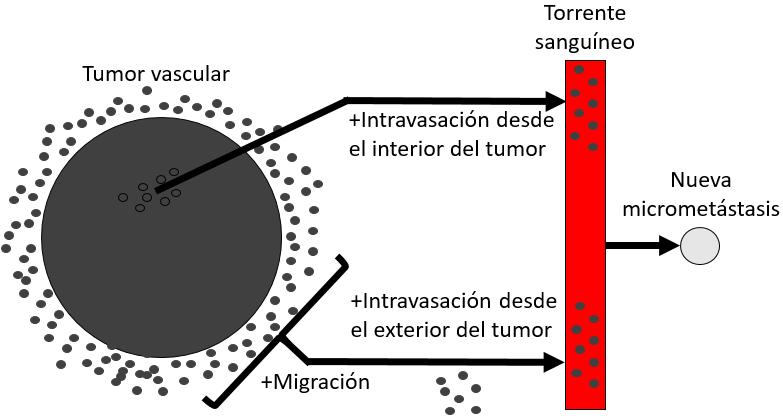
\includegraphics{img/fig-metastasis-vias.png}}
\end{center}\vspace*{-0.6cm}
\caption[Descripci\'on de las distintas rutas de la met\'astasis del c\'ancer]{Descripci\'on de las distintas rutas de la met\'astasis del c\'ancer. Las c\'elulas cancer\'igenas que presentan mutaciones que les permiten migrar a trav\'es de la ECM pueden llevar a cabo la met\'astasis despu\'es de concluir el desplazamiento desde la frontera del tumor hasta un capilar sangu\'ineo presente en los tejidos de sost\'en o desde el interior del propio tumor a trav\'es de los capilares sangu\'ineos que crecen en su interior producto de la angiog\'enesis.}
\label{fig-metastasis-vias}
\end{figure}

Cuando una c\'elula cancer\'igena penetra el sistema circulatorio est\'a expuesta a un n\'umero de peligros que pueden terminar su existencia, entre los que se encuentran principalmente las defensas del sistema inmune que pueden reconocer y destruir estas c\'elulas y el propio estr\'es mec\'anico a que son sometidas producto de su transporte a trav\'es de capilares sangu\'ineos de menor di\'ametro que la propia c\'elula. Eventualmente se adhiere a un posible punto de extravasaci\'on en el que degrada la pared del vaso sangu\'ineo y abandona el sistema circulatorio. Al igual que ocurre con la migraci\'on del c\'ancer, hasta el momento no existe modo de determinar de forma realista la probabilidad de supervivencia de la c\'elula cancer\'igena en su transporte por el sistema circulatorio ni de predecir la localizaci\'on donde dicha c\'elula abandonar\'a el torrente sangu\'ineo, ya que es un fen\'omeno sujeto a muchos procesos de naturaleza aleatoria. Como se expres\'o en la secci\'on~\ref{subsec-meta} la teor\'ia de la semilla y el sustrato es ampliamente aceptada porque permite explicar la tendencia del c\'ancer de colonizar \'organos espec\'ificos. Bas\'andonos en esta teor\'ia se a\~naden un conjunto de hip\'otesis al modelo que permiten representar la met\'astasis del c\'ancer:

\begin{itemize}
\item [XXI.] \textbf{Conexiones distantes del grafo}: \emph{Cada \'organo representado est\'a vinculado con el otro a trav\'es de las conexiones distantes existentes en el grafo subyacente. Se asume que una c\'elula que penetre el sistema circulatorio en un punto dado lo abandonar\'a en una posici\'on predeterminada, correspondientes con los destinos de las conexiones mencionadas.} \label{XXI}
\end{itemize}

La hip\'otesis XXI se apoya en la consideraci\'on que expresa que un tejido vivo puede ser representado mediante una red de mundo peque\~no, planteada en la secci\'on~\ref{subsec-hipo}. El presente modelo reproduce las localizaciones correspondientes con el \'organo donde se origin\'o el tumor y un \'organo que es colonizado de forma preferencial por el tipo de c\'ancer en cuesti\'on, pero es necesario a\~nadir a estas localizaciones una forma que representar las c\'elulas migratorias que permanecen en el interior del sistema circulatorio. La representaci\'on de este transporte a trav\'es del sistema circulatorio debe permitir reproducir la duraci\'on del trayecto y evaluar su supervivencia. 

Supongamos que se tiene una c\'elula que presenta una conexi\'on distante, y como consecuencia de dicha conexi\'on tiene la probabilidad de convertirse en un destino potencial de la met\'astasis. Para representar la migraci\'on se define un conjunto que contiene la informaci\'on correspondiente con todas las c\'elulas migratorias que est\'an viajando a trav\'es del sistema circulatorio con sus destinos. Cuando una c\'elula migratoria alcanza una posici\'on que posee una conexi\'on distante con una c\'elula del estroma que no ha sido colonizada a\'un, la c\'elula migratoria abandona su posici\'on y pasa a pertenecer al conjunto definido anteriormente. Una vez dentro de este conjunto en cada instante de tiempo se prueba su supervivencia hasta que abandone el sistema circulatorio para colonizar finalmente la posici\'on destino. Esta sucesi\'on de pasos describe a grandes rasgos la idea detr\'as de la met\'astasis, pero la posici\'on destino no tiene que ser necesariamente una c\'elula del estroma para que la c\'elula migratoria considere que es un destino viable para la met\'astasis. El destino puede ser una c\'elula del estroma, una c\'elula de un tumor o una c\'elula de una micromet\'astasis. Cada uno de estos destinos se corresponde con las distintas situaciones expuestas en la secci\'on~\ref{subsec-meta} que pueden darse cuando una c\'elula migratoria abandona el sistema circulatorio en una localizaci\'on, de ah\'i que el conjunto que contiene los posibles destinos de la met\'astasis tenga la forma ${\mathcal{E}_{met}}=\lbrace 2,3,5 \rbrace$. Si la c\'elula destino es una c\'elula de un tumor o es alguna micromet\'astasis se infiere que si la c\'elula migratoria sobrevive al transporte y extravasa satisfactoriamente, esta contribuye con la poblaci\'on de dichos tumores. Si la c\'elula destino es una c\'elula del estroma, entonces se crear\'a un nuevo foco cancer\'igeno. No obstante, est\'a fuera del alcance del presente modelo representar estas contribuciones a las poblaciones tumorales. Luego, las c\'elulas migratorias siempre penetran el sistema circulatorio si entran en contacto con una conexi\'on distante, pero solo se almacenan y eval\'uan las que tienen como destino una c\'elula del estroma o una micromet\'astasis, ya que estos tumores pueden ser eliminados por el sistema inmunitario y se debe poder representar la recreaci\'on de estos focos cancerosos. Luego se plantea la siguiente hip\'otesis: 

\begin{itemize}
\item [XXII.] \textbf{Destinos viables de la met\'astasis}: \emph{Se representan solamente las migraciones de c\'elulas cancer\'igenas hacia localizaciones que est\'an sin colonizar o que se corresponden con una micromet\'astasis. Si las localizaciones destino se corresponde con un tumor la c\'elula migratoria abandona su posici\'on y penetra el sistema circulatorio pero no se eval\'ua su transporte ni el arribo a la nueva localizaci\'on.} \label{XXII}
\end{itemize}

Como en el conjunto que representa el sistema circulatorio existen c\'elulas migratorias que poseen una misma posici\'on destino es necesario que sean actualizadas de forma secuencial para manejar las distintas situaciones de competencia, y al igual que sucede con la migraci\'on el orden de actualizaci\'on es aleatorio. La implementaci\'on del los conjunto que representa el sistema circulatorio se logra mediante un conjunto de actualizaci\'on secuencial $C_{sc}^A(G)$ en el que se almacena la informaci\'on referente a las c\'elula migratorias y su destino. Se define un nuevo par\'ametro $\xi_{sc} \in [0,1]$ que es la probabilidad de supervivencia de la c\'elula migratoria en el sistema circulatorio. La incorporaci\'on del conjunto de actualizaci\'on $C_{sc}^A(G)$ y de este par\'ametro al procedimiento de actualizaci\'on se muestra en el algoritmo~\ref{alg-update-3}. El m\'etodo encargado de actualizar las c\'elulas contenidas en el torrente sangu\'ineo se muestra en el algoritmo~\ref{alg-update-3-1}. Como se puede observar en el algoritmo~\ref{alg-update-3}, el transporte en el interior del sistema circulatorio se eval\'ua inicialmente, de forma tal que las c\'elulas que lo penetren como consecuencia de la actualizaci\'on de las c\'elulas migratorias no sean evaluadas hasta el instante de tiempo siguiente.

\begin{algorithm}[!ht]
\caption{Implementaci\'on del procedimiento de actualizaci\'on del aut\'omata celular incorporando el par\'ametro $\xi_{sc}$ y el conjunto de actualizaci\'on secuencial para las c\'elulas migratorias en el interior del sistema circulatorio $C_{sc}^A(G)$.} \label{alg-update-3}
\KwData{$G,\,C_{mig}^A(G),\,C_{sc}^A(G),\,C^S(G),\,S(n),\,\mu_{mig},\,\xi_{sc}$}
$Update$-$Migratory$-$Cells$-$In$-$Bloodstream(C_{sc}^A(G),\,\xi_{sc})$\;
$Update$-$Migratory$-$Cells(G,\,C_{mig}^A(G),\,S(n),\,\mu_{mig})$\;
$Update$-$Synchronous$-$Cells(G,\,C^S(G),S(n))$\;
\end{algorithm}

\begin{algorithm}[!ht]
\caption{Implementaci\'on del m\'etodo $Update$-$Migratory$-$Cells$-$In$-$Bloodstream$ $(C_{sc}^A(G),\xi_{sc})$ utilizado en el procedimiento de actualizaci\'on del aut\'omata celular y que se encarga de la actualizaci\'on del conjunto secuencial que contiene a las c\'elulas migratorias contenidas en el torrente sangu\'ineo.} \label{alg-update-3-1}
\KwData{$C_{sc}^A(G),\,\xi_{sc}$}
\While{$|C_{sc}^A(G)|~\neq~0$}{
	$v=Select$-$Random$-$Vertex(C_{sc}^A(G))$\;
	$w=Get$-$Target$-$Vertex(v,\,C_{sc}^A(G))$\;
	\If{$Random(0,1) \leq \xi_{sc} \wedge s(w,n) = 2$}{		
		$Create$-$New$-$Metastasis(w)$\;}
	$Remove$-$Cell$-$From$-$Bloodstream(v,\,C_{sc}^A(G))$\;}
\end{algorithm}

El algoritmo~\ref{alg-update-3-1} describe el proceso de transporte y extravasaci\'on de las c\'elulas migratorias, luego resta definir el proceso de inserci\'on en el sistema circulatorio. Como se expres\'o anteriormente existen dos posibles situaciones en las que una c\'elula migratoria penetra el torrente sangu\'ineo. Para representar la primera situaci\'on en que la c\'elula migratoria parte desde la frontera del tumor y arriba a un posible punto de intravasaci\'on, se plantea una regla del aut\'omata celular, mientras que para la segunda situaci\'on en la que una c\'elula tumoral provoca el surgimiento de una c\'elula migratoria que penetra directamente el torrente sangu\'ineo, se agregan las instrucciones necesarias al algoritmo~\ref{alg-update-3} en las l\'ineas correspondientes con la actualizaci\'on del conjunto sincronizado $C^S(G)$ para representar dicha situaci\'on. Estas modificaciones consisten en verificar la existencia de una c\'elula tumoral en presencia de una conexi\'on distante, que en caso afirmativo se a\~nade una c\'elula migratoria a la representaci\'on del torrente sangu\'ineo con el destino correspondiente. Una observaci\'on importante es que una misma c\'elula puede poseer m\'as de una conexi\'on distante producto de la aleatoriedad del proceso de reconexi\'on del modelo Watts-Strogatz. Por tanto se sigue el mismo esquema de la regla de la migraci\'on: actualizar el estado de la c\'elula mediante la aplicaci\'on de la regla de la met\'astasis y elegir de forma aleatoria el destino. 

Comenzamos definiendo la regla para la primera situaci\'on descrita anteriormente. Como se expuso en la secci\'on~\ref{subsec-migration} el final de la migraci\'on est\'a dada por la existencia de una conexi\'on distante viable para la met\'astasis en la posici\'on actual de la c\'elula migratoria. Esta condici\'on constituye el criterio de selecci\'on de la regla para la met\'astasis como se muestra a continuaci\'on:
\begin{equation}
s(v,n)=\mathcal{R}(S(v,n))= 2~~\textit{si } s(v,n)=4~\wedge~\mathcal{N}_{\mathcal{E}_{met}}^d(S(v,n))>0. \label{eq-intravasation}
\end{equation}

Se puede apreciar en la expresi\'on~(\ref{eq-intravasation}) que la regla posee un car\'acter determinista, ya que su aplicaci\'on siempre resulta en el abandono de la posici\'on por parte de la c\'elula migratoria. Al aplicarse esta regla la c\'elula migratoria pasa a pertenecer al conjunto de actualizaci\'on secuencial $C_{sc}^A(G)$ con la informaci\'on referente a su destino y con un tiempo de transporte igual a cero. Entonces definimos el proceso de selecci\'on del destino de la met\'astasis como:

\begin{definition}
\label{def-type-neighbours-2}
La funci\'on $D_{met}(v,n)$, que recibe una c\'elula migratoria $v$ y un instante de tiempo $n$, devuelve el conjunto de c\'elulas vecinas distantes de $v$ tales que su estado en el instante de tiempo $n$ est\'e contenido en el conjunto $\mathcal{E}_{met}=\lbrace 2,3,5 \rbrace$, es decir:
\begin{equation}
D_{met}(v,n) = \lbrace w~|~w \in \mathcal{N}^d(v)~\wedge~s(w,n) \in \mathcal{E}_{met} \rbrace. \label{eq-type-neighbours-2}
\end{equation}
\end{definition}

La selecci\'on de la posici\'on destino comienza evaluando la funci\'on~(\ref{eq-type-neighbours-2}) en la c\'elula $v$ en el instante de tiempo actual, obteniendo un conjunto de posibles destinos de la forma $D_{met}(v,n) = \lbrace w_1, w_2, \ldots, w_m \rbrace$ con $m={|D_{met}(v,n)|}$ para luego seleccionar uno de estos de forma aleatoria.

\begin{definition}
\label{def-dest-selection-met}
La funci\'on $d_{met}(v,n)$, que recibe una c\'elula $v$ y un instante de tiempo $n$, devuelve una c\'elula $w$ que pertenece al conjunto $D_{met}(v,n)$ y constituye el destino elegido para la met\'astasis de la c\'elula $v$. El procedimiento queda de la siguiente forma:
\begin{equation}
d_{met}(v,n) = \left\lbrace
	\begin{array}{ll}
		w_1 & \textit{con probabilidad } 1/m\\
		w_2 & \textit{con probabilidad } 1/m\\
		\vdots & \ldots\\
		w_m & \textit{con probabilidad } 1/m
	\end{array}
\right., \label{eq-dest-selection-met}
\end{equation}
donde $D_{met}(v,n)= \lbrace w_1,w_2,\ldots,w_m \rbrace$ con $m = |D_{met}(v,n)|$. Se puede apreciar que todos los destinos viables poseen la misma probabilidad de ser elegidos.
\end{definition}

Finalmente, las modificaciones al algoritmo~\ref{alg-update-3} para representar el surgimiento de una c\'elula migratoria que penetra el sistema circulatorio desde el interior del propio tumor se realizan de forma an\'aloga a las concebidas para representar la migraci\'on, utilizando con este fin un nuevo conjunto de actualizaci\'on sincronizado $C_{tum}^S(G)$ que contiene a las c\'elulas cancer\'igenas que pertenecen al interior de alg\'un tumor vascular y que est\'an en presencia de una conexi\'on distante. El m\'etodo para la actualizaci\'on de estas c\'elulas es el siguiente: por cada c\'elula del conjunto se eval\'ua la probabilidad del surgimiento de una c\'elula descendiente migratoria cuya expresi\'on se expone en~(\ref{eq-migrant-2}) y~(\ref{eq-migrant-3}), y si ocurre la aparici\'on de dicha c\'elula, se coloca en el conjunto de actualizaci\'on secuencial $C_{sc}^A(G)$ con su destino seleccionado de forma aleatoria de entre los posibles. La necesidad de incluir este mecanismo para el surgimiento de c\'elulas migratorias est\'a dada por la representaci\'on del sistema circulatorio, impidiendo que pueda representarse propiamente mediante una regla del aut\'omata. El procedimiento de actualizaci\'on incorporando el nuevo conjunto de actualizaci\'on y el m\'etodo correspondiente se muestran en los algoritmos~\ref{alg-update-4} y~\ref{alg-update-4-1} respectivamente. 

\begin{algorithm}[!ht]
\caption{Implementaci\'on del procedimiento de actualizaci\'on del aut\'omata celular incorporando el conjunto de actualizaci\'on sincronizado para las c\'elulas migratorias que penetran el sistema circulatorio desde una conexi\'on distante en el interior de un tumor $C_{tum}^S(G)$.} \label{alg-update-4}
\KwData{$G,\,C_{mig}^A(G),\,C_{sc}^A(G),\,C_{tum}^S(G),\,C^S(G),\,S(n),\,\mu_{mig},\,\xi_{sc},\,N_{tum},\,n$}
$Update$-$Migratory$-$Cells$-$In$-$Bloodstream(C_{sc}^A(G),\,\xi_{sc})$\;
$Update$-$Migratory$-$Cells(G,\,C_{mig}^A(G),S(n),\,\mu_{mig})$\;
$Update$-$Tumor$-$Migratory$-$Cells(G,\,C_{tum}^S(G),\,C_{sc}^A(G),\,S(n),\,N_{tum},\,n)$\;
$Update$-$Synchronous$-$Cells(G,\,C^S(G),S(n))$\;
\end{algorithm}

\begin{algorithm}[!ht]
\caption{Implementaci\'on del m\'etodo $Update$-$Tumor$-$Migratory$-$Cells(G,S(n),$  $C_{tum}^S(G),C_{sc}^A(G),\,N_{tum},\,n)$ utilizado en el procedimiento de actualizaci\'on del aut\'omata celular y que se encarga de la actualizaci\'on del conjunto sincronizado que contiene a las c\'elulas tumorales que est\'an en presencia de una conexi\'on distante y cuya descendencia migratoria posee la probabilidad de intravasar al interior del sistema circulatorio.} \label{alg-update-4-1}
\KwData{$G,\,S(n),\,C_{tum}^S(G),\,C_{sc}^A(G),\,N_{tum},\,n$}
\For{$v \in C_{tum}^S(G)$}{
	$p=Get$-$Probability(n - N_{tum}[tumor(v)])$\;
	\If{$Random(0,1) \leq p$}{
		$d=Select$-$Destiny$-$Vertex(v,\,S(n),\,G)$\;
		$Add$-$Cell$-$To$-$Bloodstream(v,\,d,\,C_{sc}^A(G))$\;}}
\end{algorithm}